\documentclass{vgtc}                          % final (conference style)

\ifpdf%                                % if we use pdflatex
  \pdfoutput=1\relax                   % create PDFs from pdfLaTeX
  \pdfcompresslevel=9                  % PDF Compression
  \pdfoptionpdfminorversion=7          % create PDF 1.7
  \ExecuteOptions{pdftex}
  \usepackage{graphicx}                % allow us to embed graphics files
  \DeclareGraphicsExtensions{.pdf,.png,.jpg,.jpeg} % for pdflatex we expect .pdf, .png, or .jpg files
\else%                                 % else we use pure latex
  \ExecuteOptions{dvips}
  \usepackage{graphicx}                % allow us to embed graphics files
  \DeclareGraphicsExtensions{.eps}     % for pure latex we expect eps files
\fi%

%% it is recomended to use ``\autoref{sec:bla}'' instead of ``Fig.~\ref{sec:bla}''
%\graphicspath{{figures/}{pictures/}{images/}{./}} % where to search for the images
 \usepackage[utf8]{inputenc}
 
\usepackage{microtype}                 % use micro-typography (slightly more compact, better to read)
\PassOptionsToPackage{warn}{textcomp}  % to address font issues with \textrightarrow
\usepackage{textcomp}                  % use better special symbols
\usepackage{mathptmx}                  % use matching math font
\usepackage{times}                     % we use Times as the main font
\renewcommand*\ttdefault{txtt}         % a nicer typewriter font
\usepackage{cite}                      % needed to automatically sort the references
\usepackage{tabu}                      % only used for the table example
\usepackage{booktabs}                  % only used for the table example

\onlineid{0}

\vgtccategory{Research}

\vgtcinsertpkg


\title{Learning PAC}

\author{Andres J. Montenegro Bello\thanks{e-mail: montenegroandresj@gmail.com}\\      \scriptsize GitHub : AndresJuniorMontenegro%
\and Raul Huaman Pajares \thanks{e-mail: rahuamanpa@gmail.com }\\ %
     \scriptsize GitHub : rhuamanpa\\
\and Repositorio \\
     \scriptsize https://github.com/rhuamanpa/Pac-Learning
}

%% Abstract section.
\abstract{ We will analize PAC learning, the type of uses that we can apply with PAC learning with machine learning and show some samples used by big companies like Facebook and Youtube to make incomes at the same time we will make a project using PAC learning using python that will recognize some facial gestures.%
} % end of abstract

%%%%%%%%%%%%%%%%%%%%%%%%%%%%%%%%%%%%%%%%%%%%%%%%%%%%%%%%%%%%%%%%
%%%%%%%%%%%%%%%%%%%%%% START OF THE PAPER %%%%%%%%%%%%%%%%%%%%%%
%%%%%%%%%%%%%%%%%%%%%%%%%%%%%%%%%%%%%%%%%%%%%%%%%%%%%%%%%%%%%%%%%

\begin{document}

\firstsection{Introduction}

\maketitle

%% \section{Introduction} %for journal use above \firstsection{..} instead
La probabilidad aproximada correcta (PAC), propuesta por L.Valiant,
es un marco de referencia estatico para aprender usar datos de entrenamiento.
\\
\\
En su forma mas simple y para un modelo tipico de tarea, la teoria
del aprendizaje PAC intentan relacionar, precision y confianza 
estadistica del modelo al numero de ejemplos de entrenamientos 
usados.
\\
\\
Uno de los conceptos más importantes en este sentido es medir la
complejidad de una clase de hipótesis $H$. En cualquier modelo de
aprendizaje automático, el objetivo final es encontrar una clase de
hipótesis que logre una alta precisión en el conjunto de
entrenamiento y que tenga un bajo error de generalización en el conjunto
de prueba. Para esto, requerimos que la clase de hipótesis $H$ se
aproxime al concepto de clase $C$ que determina las etiquetas para la
distribución $D$. Como tanto $C$ como $D$ son desconocidos, tratamos
de modelar $H$ en base al conjunto de muestras conocido $S$ y sus etiquetas.

\textbf{Generalizacion del error: }
El error de generalización de una hipótesis $h$ es la expectativa del
error en una muestra $x$ elegida de la distribución $D$.

\textbf{Error empirico: }
Esta es la media del error de la hipótesis $h$ en la muestra $S$ del 
tamaño $m$.

Habiendo definido el error de generalización y el error empírico de
esta manera, podemos establecer el objetivo del aprendizaje de la
siguiente manera.
\newline
\newline
\textit{El objetivo del aprendizaje es tener el error empírico
aproximado al error de generalización con alta probabilidad.}
\newline
\newline
Este tipo de marco de aprendizaje se conoce como Aprendizaje PAC
(Probablemente Aproximadamente Correcto). Formalmente, una clase de
concepto $C$ es $PAC-aprendible$ si hay algún algoritmo $A$ para el 
cual el error de generalización en una muestra $S$ derivado de la 
distribución $D$ es muy bajo (menor que $\epsilon$) con alta 
probabilidad (mayor que $1- \delta$). En otras palabras, podemos decir que para una
clase apta para PAC, la precisión es alta con buena confianza.
\\
\\
Se adjuntara una imagen en la cual dara una descripcion general del aprendizaje PAC.
\\
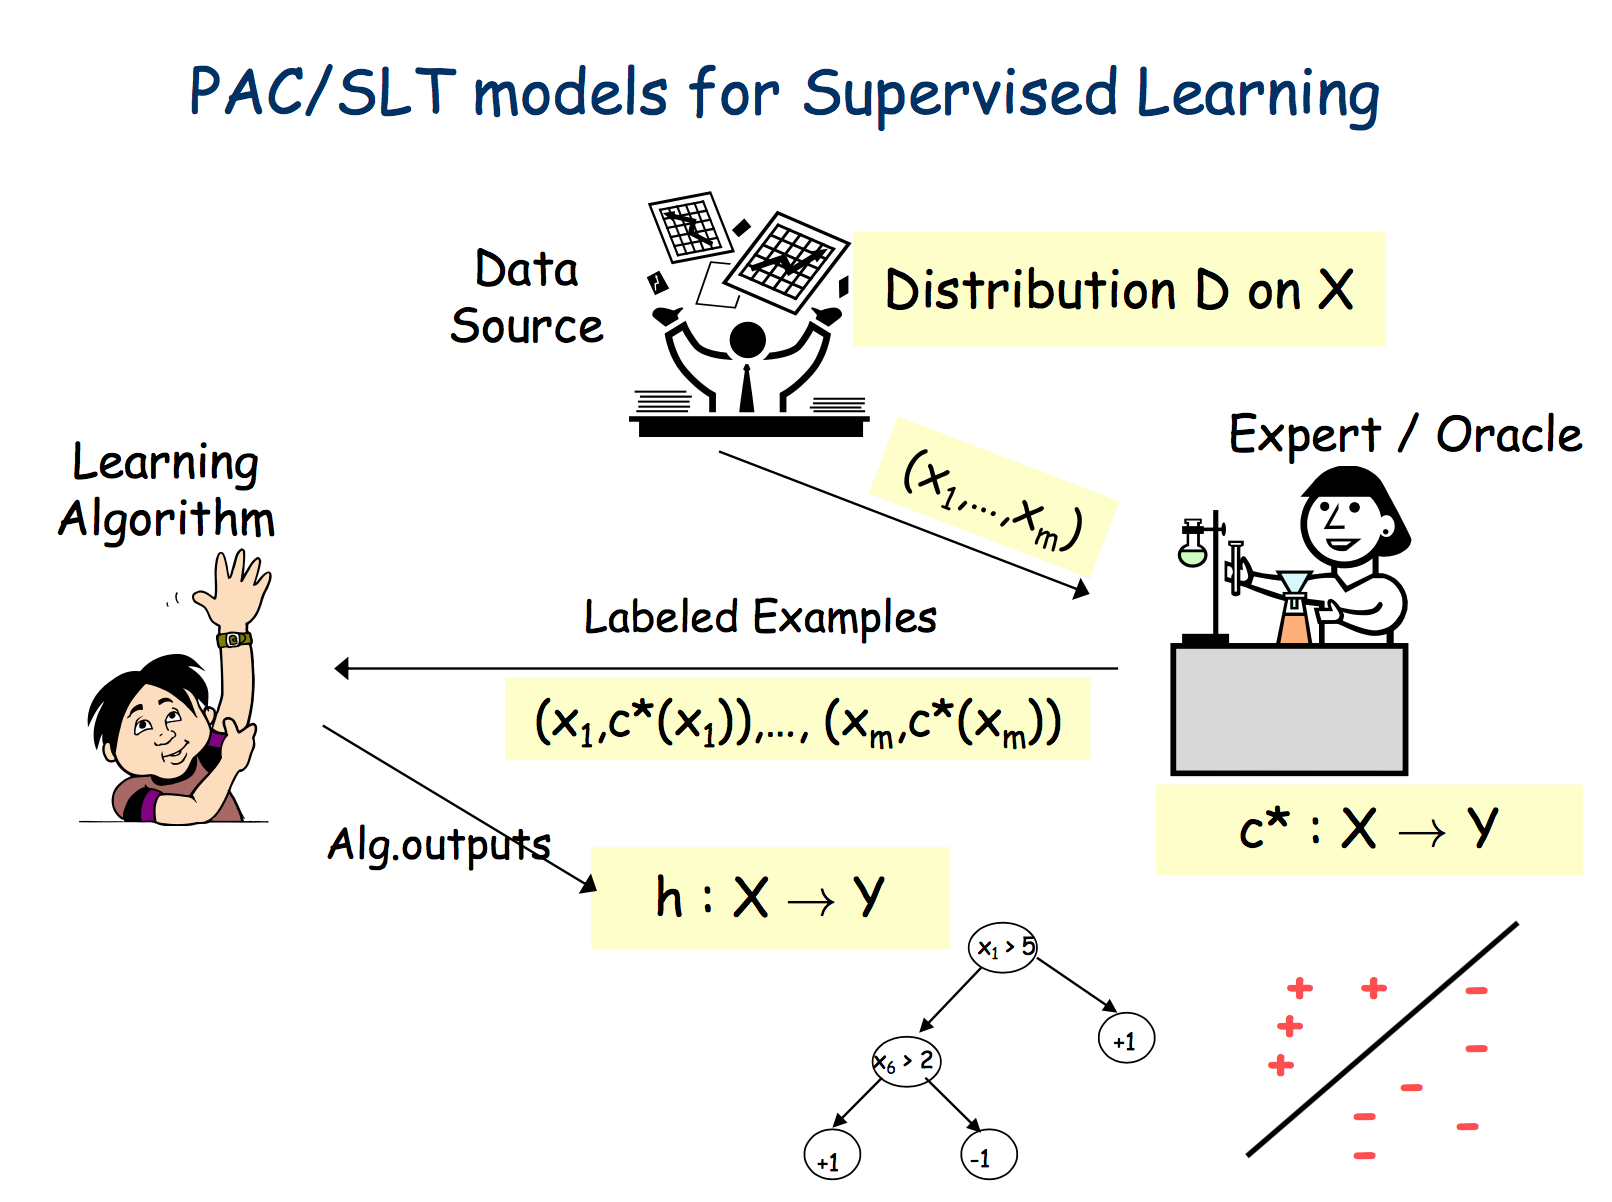
\includegraphics[scale=0.15]{pac.png} 
\section{Estado del arte}

El aprendizaje PAC( aprendizaje correcto probablemente aproximado) como su
nombre lo dice generara probables situaciones para dar un resultado
correcto aproximado, esta ciencia es una similitud o podemos decir una
rama del machine learning y el deep learning, sus usos son muy dinamicos y
eficaces, actualmente se utiliza como herramienta muy util veamos 3
ejemplos:
\newline
\newline
\textbf{Identificación de temas: }
Clasificación multi-etiqueta de medio de articulos impresos deducido
de una base de datos.
\newline
\newline
La data fue recolectada desde el Mayo del 2013 hasta Setiembre del 2013,
\newline
\newline
Los articulos fueron manualmente segmentados.
\newline
\newline
El texto de los articulos es representado usando \textit{"Una mochila de
palabras modelo "}.
\newline
\newline
Esta base de datos cuenta con $301 561$ atributos numericos, $213$ tipo de
etiqueta y $99 780$ articulos, los cuales $64 857$ fueron data de 
entrenamiento y $34 923$ fueron data de prueba, el objetivo es predecir 
las etiquetas relevantes del conjunto de data de prueba.
\newline
\newline
Se adjunta el link del conjunto de data:
\newline
\newline
\url{https://www.kaggle.com/c/wise-2014/data}
\newline
\newline

\textbf{Recomendación de peliculas: }
Sistema utilizado para predecir la afluencia que tendra una pelicula y su calificacion 
global, determinada por la calificacion previa a peliculas con similar caracteristica 
o etiqueta sacada de una base de datos ya sea de \textit{Netflix} o \textit{Movie Lens}
\newline
\newline
Se adjuntara los links de la base de datos de dichas plataformas de peliculas:

\textit{Netflix: \\}  \url{https://www.netflixprize.com/leaderboard.html}
\newline
\newline
\textit{Movie Lens:\\ } \url{https://grouplens.org/datasets/movielens/}
\newline
\newline

\textbf{Video resumen: }
Selecciona semanticamente las partes más importantes de un video
debido a una base de datos muy grande de metricas en la plataforma 
de $YOUTUBE$, esto es usado como grandes compañias como \textit{Facebook y Youtube}, para que puedan insertar la publicidad
en las partes mas relevantes del video subido y asi más probabilidad
de que puedan ver la publicidad.
\newline
\newline
Se adjunta la data de \textit{Youtube} y es : \newline \newline
\url{https://research.google.com/youtube8m/index.html}


\section{Diseño del experimento}

Se diseñara un experimento en la cual se capturara una imagen
y este reconocera ciertos gestos faciales.
\\
\\
Debido a un conjunto de patrones establecidos.
\\
\\
Se implementara con el lenguaje de programación \textit{Python.}



\bibliography{template}
\end{document}
